\documentclass[10pt]{beamer}

\usetheme{metropolis}
\usepackage{appendixnumberbeamer}

\usepackage{booktabs}
\usepackage[scale=2]{ccicons}

\usepackage{pgfplots}
\usepgfplotslibrary{dateplot}

\usepackage{xspace}
\newcommand{\themename}{\textbf{\textsc{metropolis}}\xspace}

\title{Wild Binary Segmentation}
\subtitle{A Monte Carlo-like approach to localizing changepoints in data}
\date{\today}
\author{Magnus Berg Sletfjerding}
% \institute{Center for modern beamer themes}
% \titlegraphic{\hfill\includegraphics[height=1.5cm]{logo.pdf}}

\begin{document}

\maketitle

% \begin{frame}{Table of contents}
%   \setbeamertemplate{section in toc}[sections numbered]
%   \tableofcontents[hideallsubsections]
% \end{frame}

\begin{frame}[t]{The Problem}
  Let's say we have a noisy time series data.

  \begin{columns}
  \begin{column}[T]{0.48\textwidth}
    \begin{itemize}
      \item Financial data
      \item Student satisfaction over time
      \item Traffic Data
      \item Biomolecular activity
    \end{itemize}
  \end{column}
  \hfill
  \begin{column}[T]{0.48\textwidth}
  We would prefer to separate this data into separate chunks that are easier to work with.
  But how?!
  \end{column}
  \end{columns}


  \begin{figure}
    \only<2>{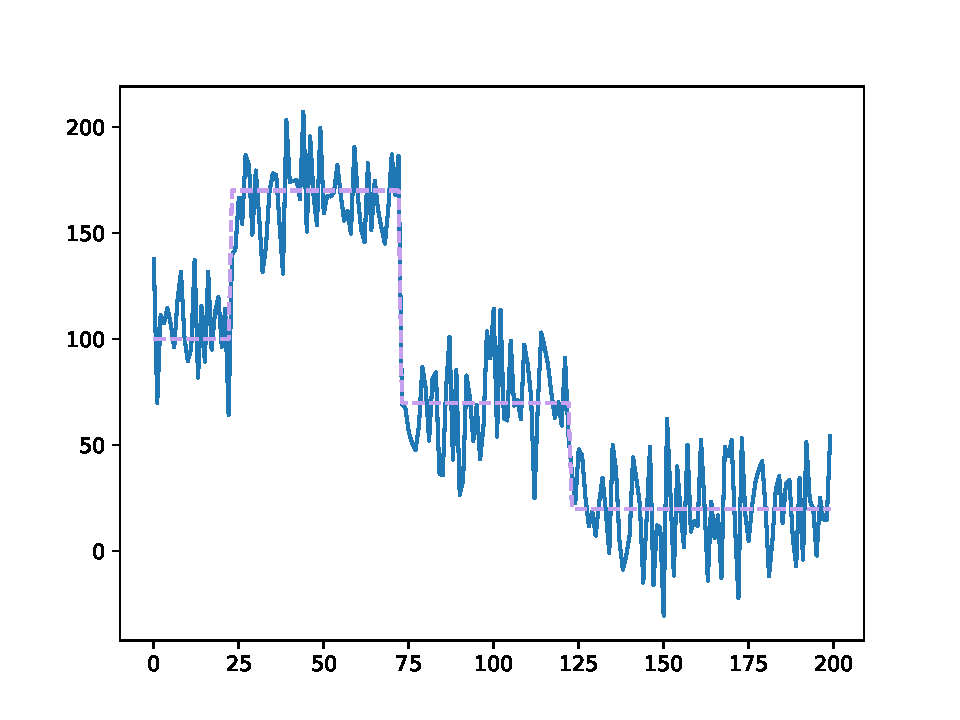
\includegraphics[width=0.6\textwidth]{../wsb_figures/onlytrace.pdf}}
    \only<3->{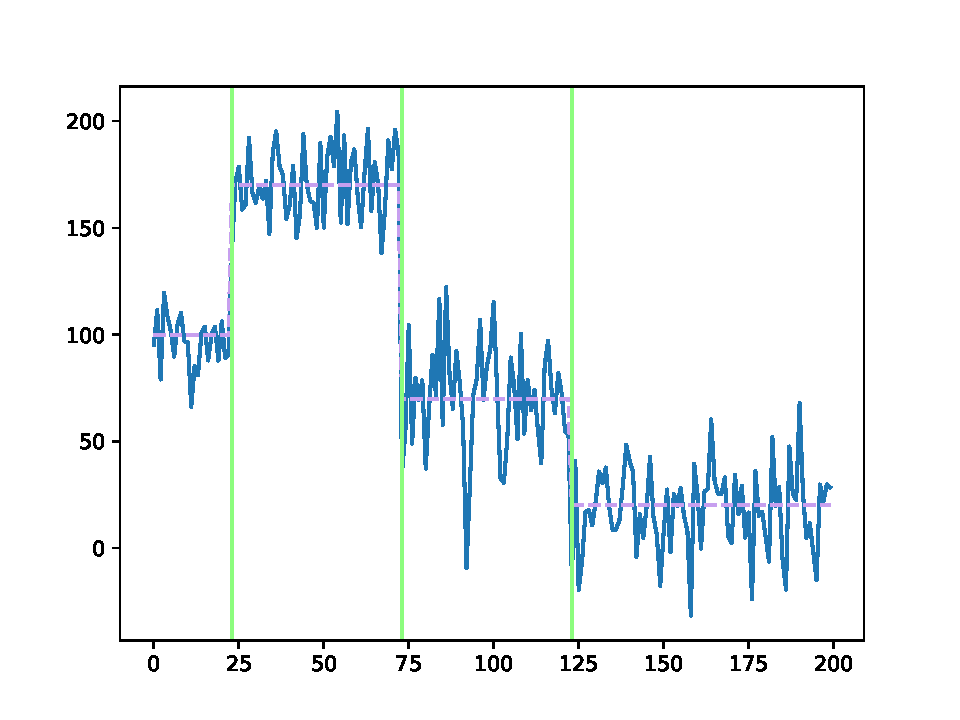
\includegraphics[width=0.6\textwidth]{../wsb_figures/trace.pdf}}

  \end{figure}

\end{frame}
%--- Next Frame ---%
\begin{frame}[t]{Binary Segmentation}
  This is the classical way of finding changepoints in data.
  \begin{figure}
    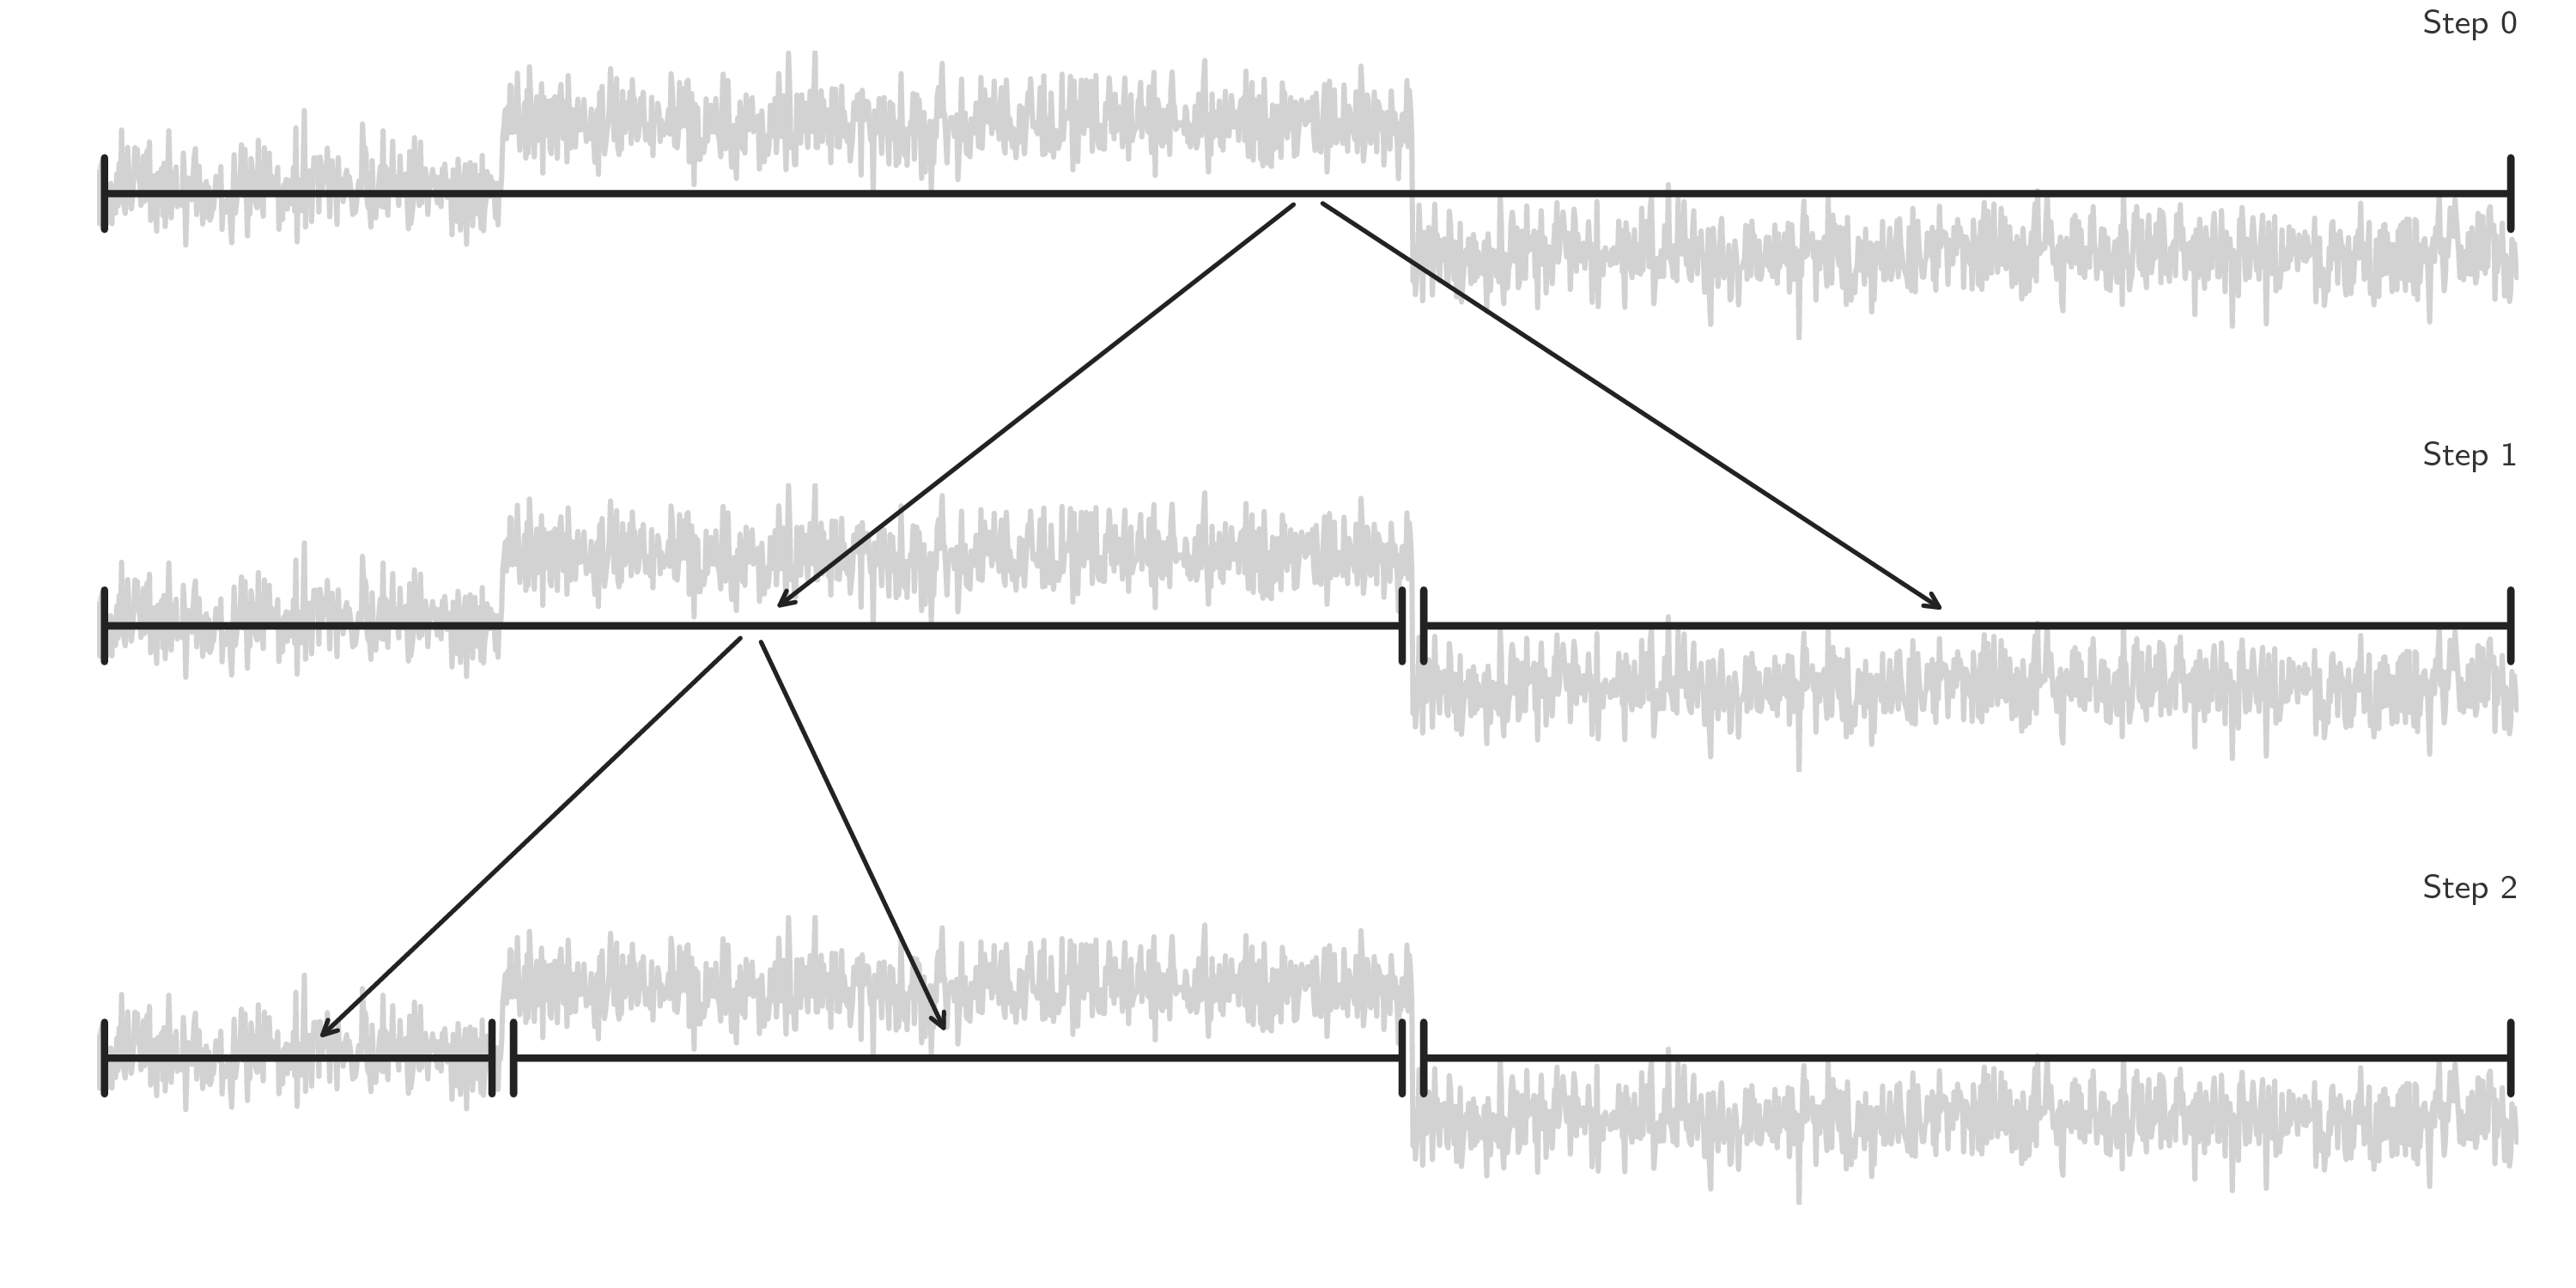
\includegraphics[width=\textwidth]{../wsb_figures/schema_binseg.png}
  \end{figure}
  It's quick, easy to understand, and easy to conceptualize.
\end{frame}
%--- Next Frame ---%

\begin{frame}[t]{Binary Segmentation - math}
Assume that our data can be like so:
\[X_t = f_t+\varepsilon_t,  t = 1, \textellipsis,T  \]
where \(f_t\) is a one-dimensional signal which has an unknown number of changepoints  \(N\), with unknown locations  \(\eta_1, \textellipsis, \eta_N\), and  \(\varepsilon_t\) is a normal random variable centered at 0.

Binary Segmentation maximizes this statistic:
\[
\tilde{X}^{b}_{s,e} = \sqrt{\frac{e - b}{n(b-s+1)}} \sum_{t=s}^{b}X_t - \sqrt{\frac{b-s+1}{n(e - b)}} \sum_{t=b+1}^{e}X_t
\]
where \( s \leq b < e \) and \( n = e - s + 1 \).

What are we left with?
The \textbf{most likely changepoint,} \(b_0\)

\end{frame}
%--- Next Frame ---%

\begin{frame}[t]{So Binary Segmentation is perfect?}
  Not quite.
  Sometimes, the test statistic used can end up being maximized at places where there is no changepoint!!

  \begin{figure}
    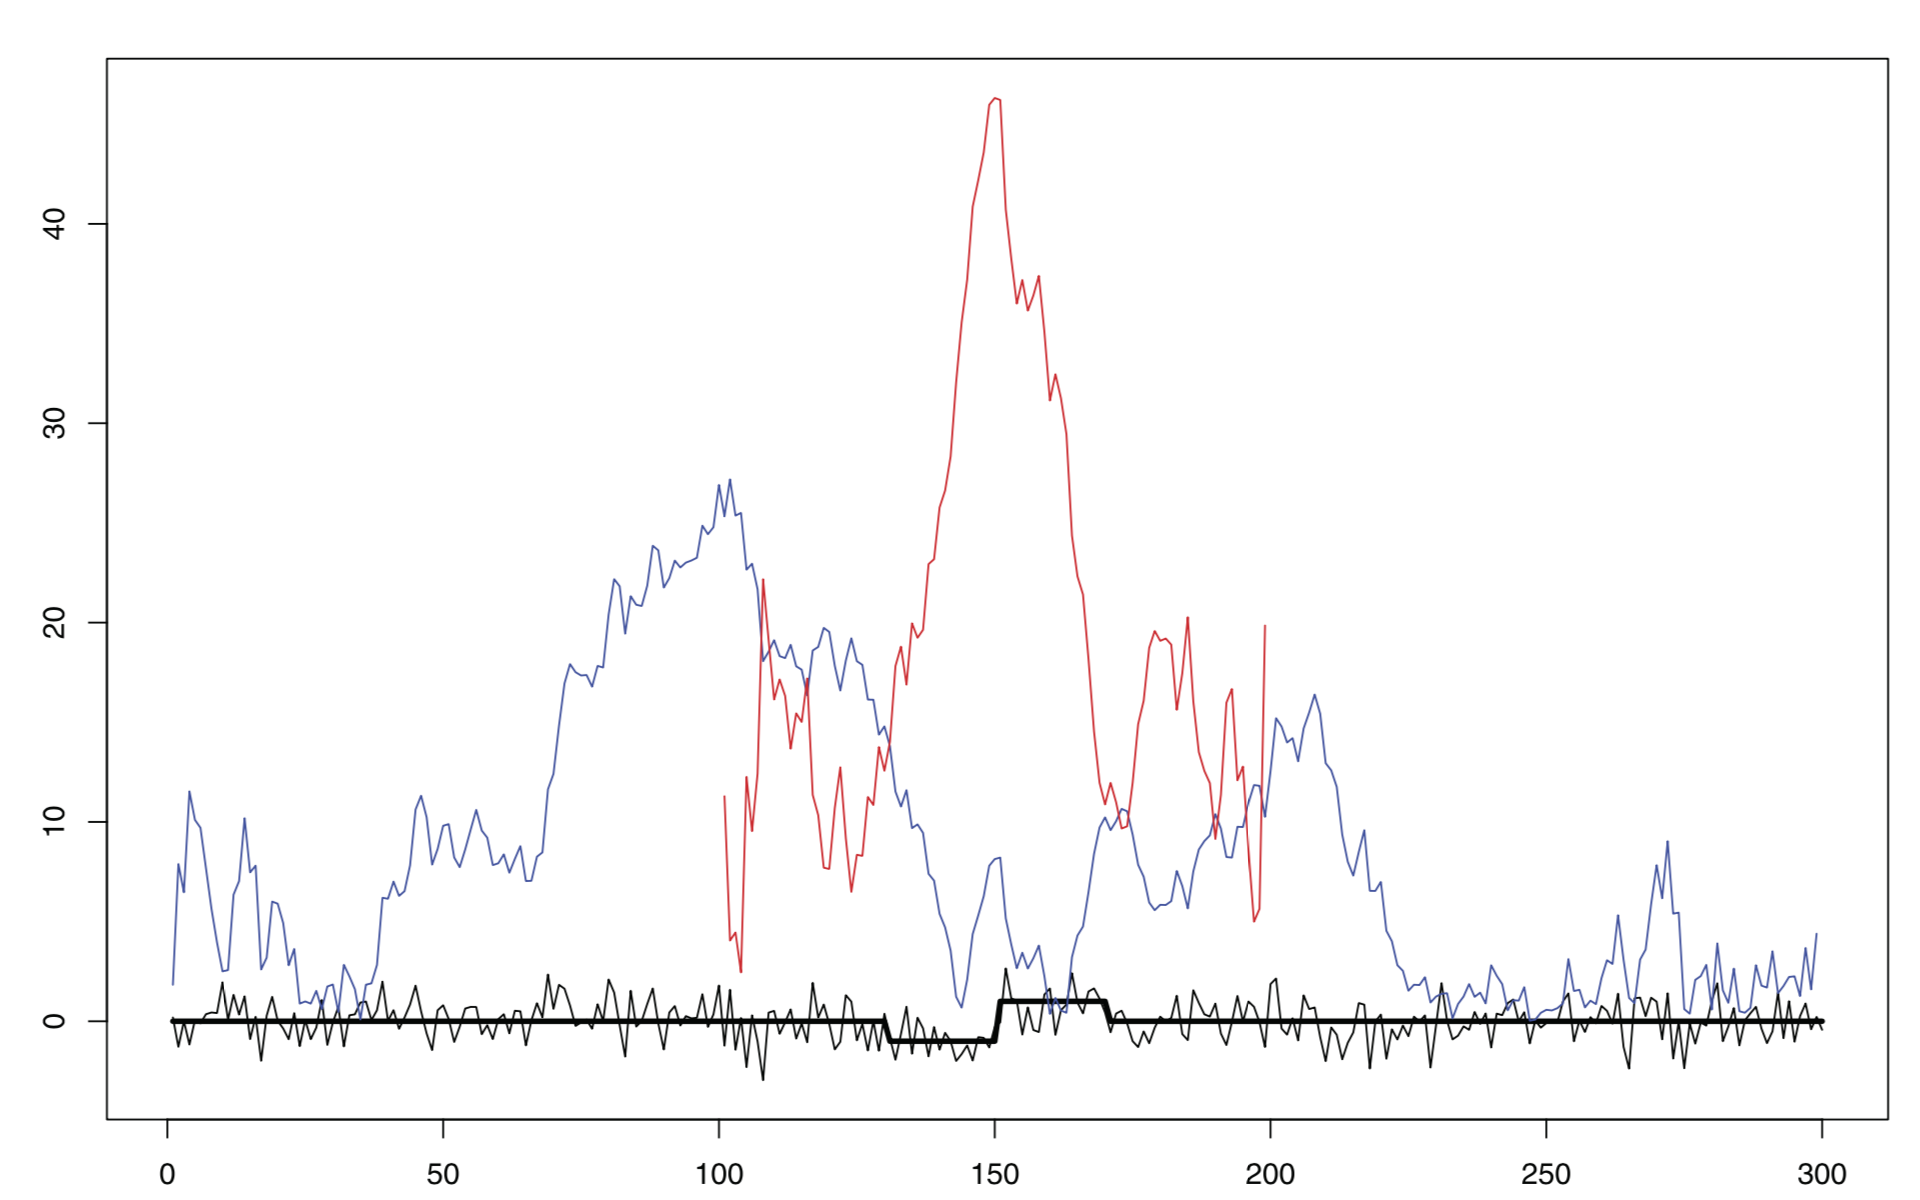
\includegraphics[width=0.8\textwidth]{../report/bsisBS.png}
  \end{figure}
  Hopefully there will be a better method in the next slide!
\end{frame}
%--- Next Frame ---%


\begin{frame}[t]{Wild Binary Segmentation}
Before doing any Binary Segmentation, make a set \(F_T^M\) of $M$ randomly sampled \textbf{intervals} $[s_m,e_m], m=1,\textellipsis,M$ where $[s_m,e_m]$ have been drawn from ${1,\textellipsis, M}$.

Once that's done, do binary segmentation on ALL the intervals, but only choose the \(b_0^m\) that completely maximizes \(\tilde{X}^{b}_{s,e}\)

Higher chance that the fit will find the ''right'' values.
\end{frame}
%--- Next Frame ---%

\begin{frame}[t]{An example}
\begin{columns}
\begin{column}[T]{0.55\textwidth}
\begin{itemize}
  \item I generated some data to work on, and implemented the two algorithms
  \item This looks more or less like what I work with on the daily
  \item Normal Binary Segmentation does not find the third(last) changepoint
  \item Wild Binary Segmentation (1000 iterations) found the true changepoints for the most part
\end{itemize}
\end{column}
\hfill
\begin{column}[T]{0.45\textwidth}
  \begin{figure}
    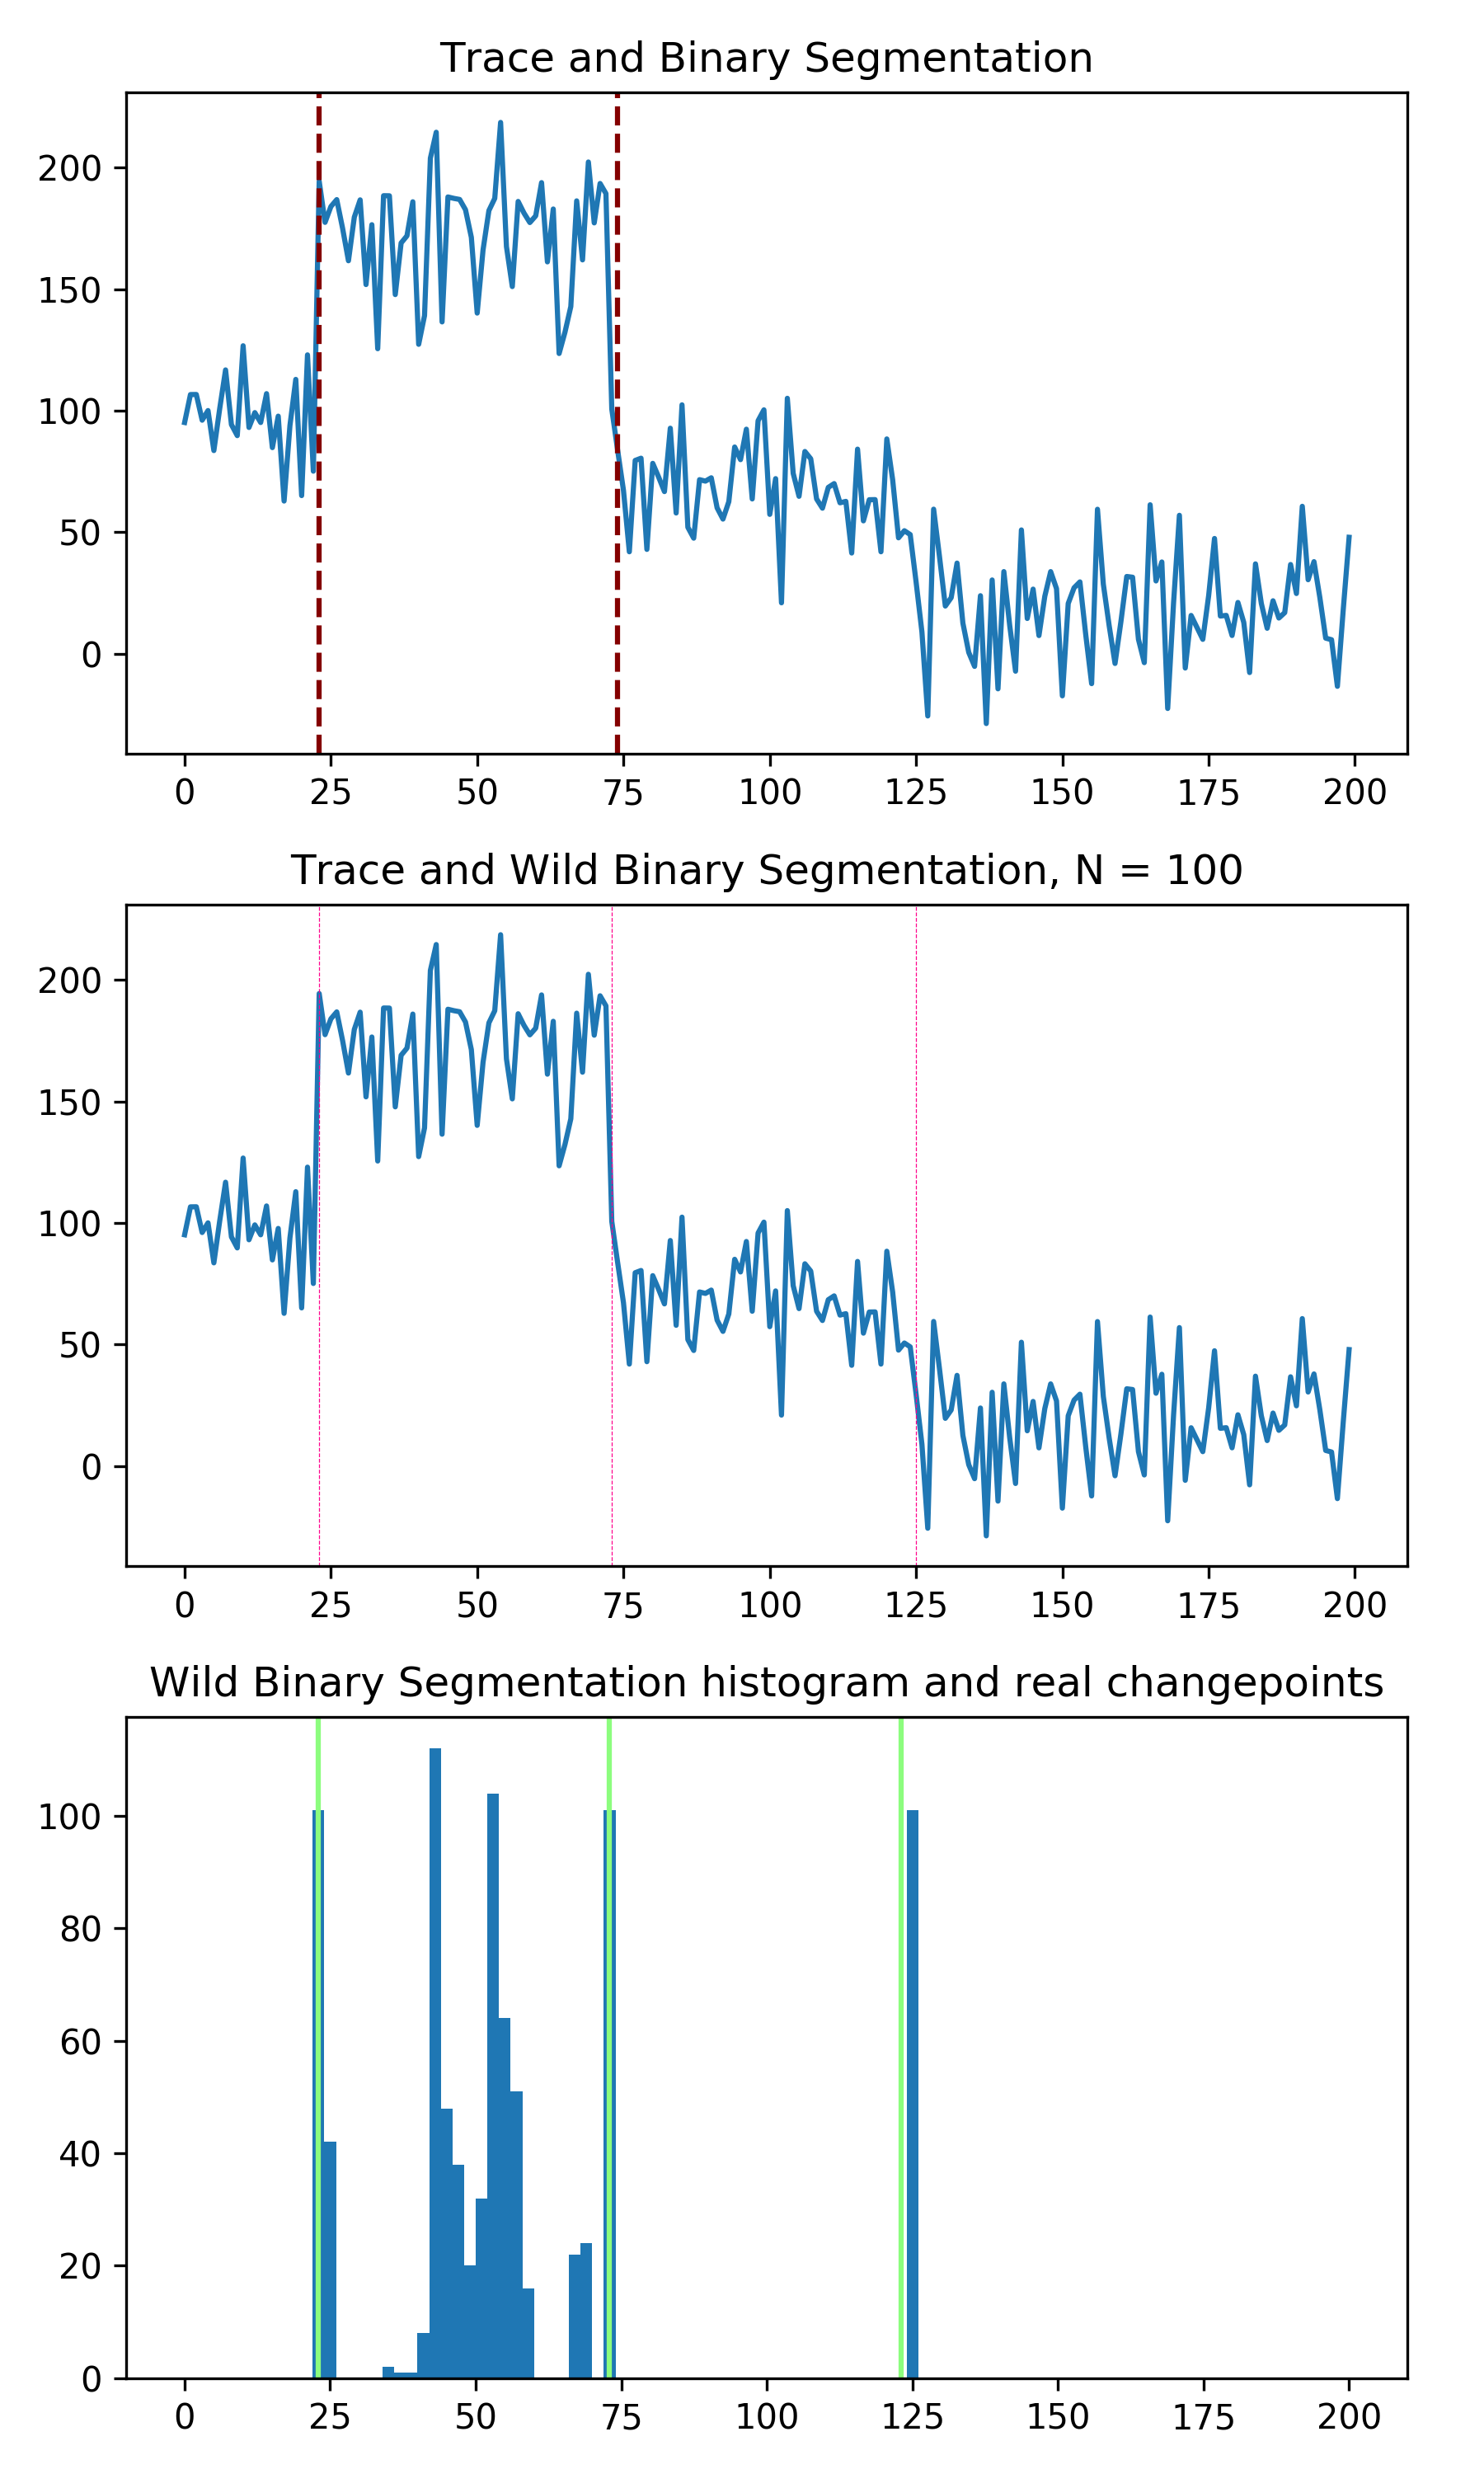
\includegraphics[width = 4.5cm]{../wsb_figures/simulation.png}
  \end{figure}
\end{column}
\end{columns}

\end{frame}
%--- Next Frame ---%

\begin{frame}[t]{Conclusion}
\begin{itemize}
  \item \(WBS > BS \)
  \item Implementing algorithms yourself is hard
  \item BS is implemented in the \texttt{ruptures} package
  \item No WBS in Python 3.7
\end{itemize}

\end{frame}
%--- Next Frame ---%


\end{document}
